\section{Evaluation}\label{sec:eval}

We evaluate \( \tool \) based on the following four research questions:
\begin{itemize}[leftmargin=0.5cm]
\item RQ1. \textbf{Effectiveness:} Does \( \tool \) effectively reduce
manual efforts in extracting the syntax and semantics from existing
ECMAScript specifications? 
\item RQ2. \textbf{Correctness:} Do the extracted syntax and semantics
from ECMAScript 2020 behave correctly?
\item RQ3. \textbf{Adaptability:} Is \( \tool \) applicable to
incomplete feature proposals?
\item RQ4. \textbf{Usefulness:} Does \( \tool \) detect any
specification errors?
\end{itemize}

\subsection{Effectiveness}

\begin{figure}[t]
  \[
    \begin{array}{c?r|r|r|r|r?r}
      \textbf{Version}
      & \multicolumn{1}{c|}{\textbf{2016}}
      & \multicolumn{1}{c|}{\textbf{2017}}
      & \multicolumn{1}{c|}{\textbf{2018}}
      & \multicolumn{1}{c|}{\textbf{2019}}
      & \multicolumn{1}{c?}{\textbf{2020}}
      & \multicolumn{1}{c}{\textbf{avg.}}\\\toprule
      \text{\# Lexical prod.}
      & \text{78}
      & \text{78}
      & \text{78}
      & \text{81}
      & \text{81}
      & \text{79.2}\\\hline
      \text{\# Syntactic prod.}
      & \text{157}
      & \text{167}
      & \text{167}
      & \text{174}
      & \text{175}
      & \text{168}\\
    \end{array}
  \]
  \[
    \begin{array}{c|r|r|r|r?r}
      \textbf{Old version}
      & \multicolumn{1}{c|}{\textbf{2016}}
      & \multicolumn{1}{c|}{\textbf{2017}}
      & \multicolumn{1}{c|}{\textbf{2018}}
      & \multicolumn{1}{c?}{\textbf{2019}}
      & \multirow{2}{*}{\textbf{avg.}}\\\cline{1-5}
      \textbf{New version}
      & \multicolumn{1}{c|}{\textbf{2017}}
      & \multicolumn{1}{c|}{\textbf{2018}}
      & \multicolumn{1}{c|}{\textbf{2019}}
      & \multicolumn{1}{c?}{\textbf{2020}}
      & \\\toprule
      \Delta \; \text{\# Lexical prod.}
      & \text{3}
      & \text{5}
      & \text{6}
      & \text{0}
      & \text{4.7}\\\hline
      \Delta \; \text{\# Syntactic prod.}
      & \text{140}
      & \text{15}
      & \text{8}
      & \text{2}
      & \text{55}\\
    \end{array}
  \]
  \caption{Number of productions in specifications,
from \textit{all} of which \( \tool \) automatically generated parsers}
  \label{fig:syntax-all-version}
\end{figure}

\begin{figure}[t]
  \centering
  \begin{subfigure}{0.23\textwidth}
    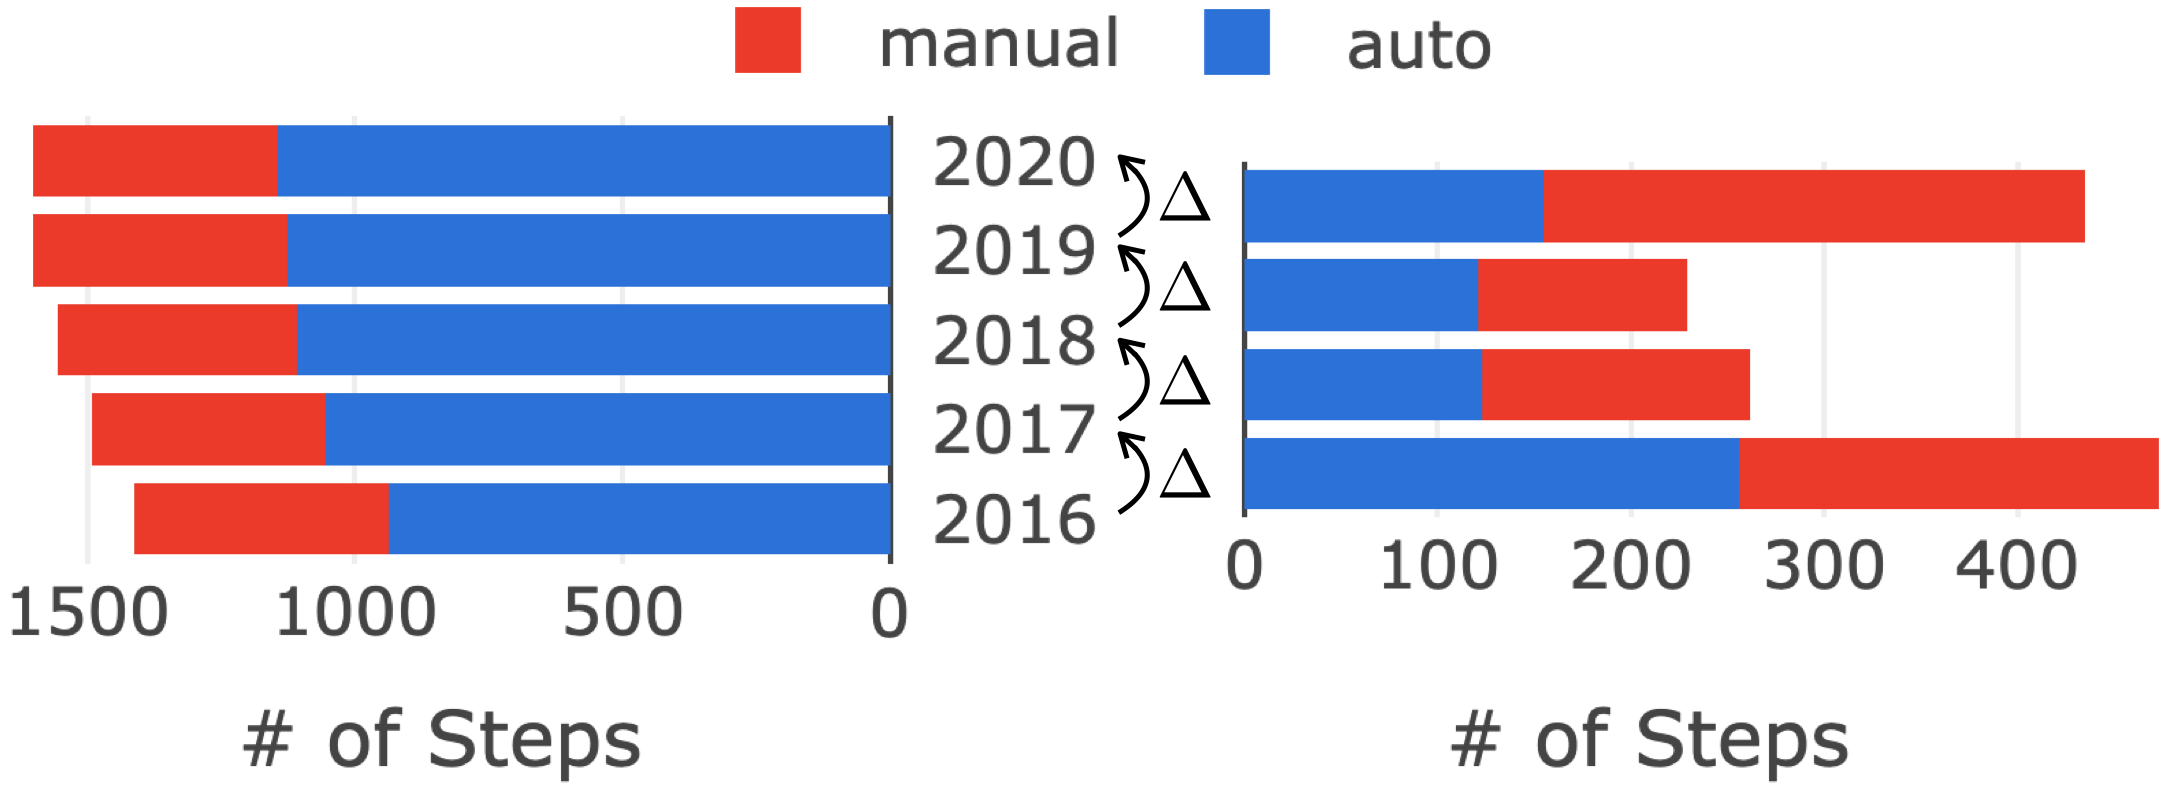
\includegraphics[width=\textwidth]{img/all-version-sem.png}
    \caption{Results for different versions}
    \label{fig:semantics-all-version}
  \end{subfigure}
  \hfill
  \begin{subfigure}{0.20\textwidth}
    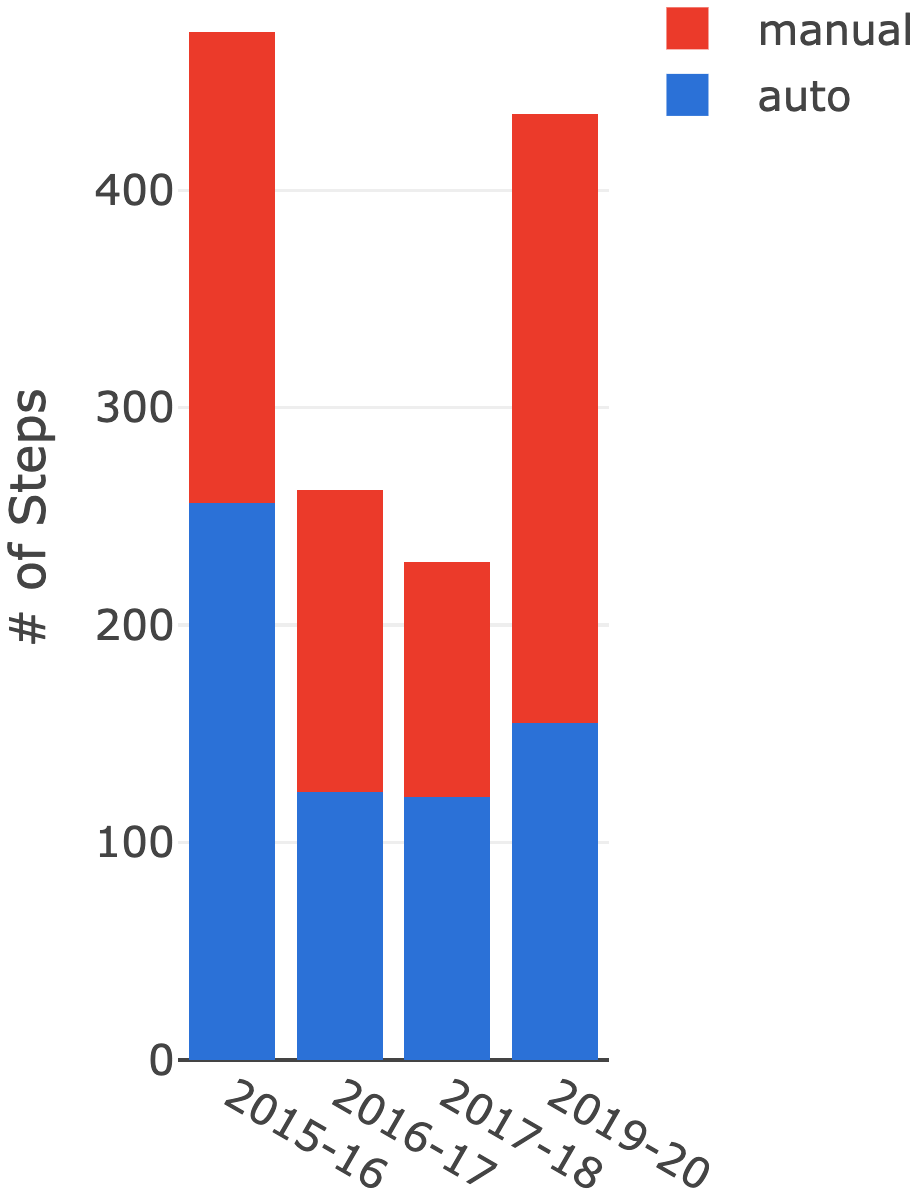
\includegraphics[width=\textwidth]{img/all-version-sem-delta.png}
    \caption{Results for differences between versions}
    \label{fig:semantics-all-version-delta}
  \end{subfigure}
  \caption{Number of abstract algorithms in specifications, from which
\( \tool \) generated the JavaScript semantics}
  \label{fig:all-version}
\end{figure}

We evaluate the effectiveness of \( \tool \) by applying it to the
most recent five versions of the ECMAScript specifications, ECMAScript
2016 to 2020.  We measured for how many grammar productions and
abstract algorithms \( \tool \) automatically generates parsers and
semantics, respectively, in two respects: 1) in each version and 2) in
each difference between adjacent versions.

For syntax, we measured the number of grammar productions for which
\textsf{Parser Generator} automatically generated parsers.  As summarized in
Figure~\ref{fig:syntax-all-version}, the average numbers of lexical and
syntactic grammar productions are \inred{XX} and \inred{XXX}, respectively.
In addition, the average numbers of annually updated lexical and
syntactic grammar productions between adjacent versions are \inred{X}
and \inred{XX}, respectively.  We report that \( \tool \)
automatically generated parsers for \textit{all} the productions.

For semantics, we measured the number of abstract algorithms that
\textsf{Algorithm Compiler} with the compile rules described in
Section~\ref{sec:impl} automatically covered.
Figure~\ref{fig:all-version} shows that \( \tool \) could
automatically extract semantics with the \inred{XX\%} success rate on
average for existing specifications, and \inred{XX\%} for changed or
newly defined algorithms.  Thus, we believe that \( \tool \) effectively
reduces the efforts to extract the syntax and semantics of JavaScript
not only for developing them from scratch, but also for updating
existing ones.

\subsection{Correctness}
\begin{table}[t]
  \centering
  \caption{Testing results of Test262 for ECMAScript 2020}
  \label{table:test262}
  \begin{tabular}{lr}\toprule
    \belowrulesepcolor{gainsboro}
    \rowcolor{gainsboro} \textbf{All tests262 Tests} & \textbf{36,794}\\
    \aboverulesepcolor{gainsboro}\midrule
    Annexes/Internationalisation & 1,774\\\hdashline
    In-progress features & 5,803\\\midrule
    \belowrulesepcolor{gainsboro}
    \rowcolor{gainsboro} \textbf{ECMAScript 2020 Tests} & \textbf{29,217}\\
    \aboverulesepcolor{gainsboro}\midrule
    Non-strict mode tests & 1,064\\\hdashline
    Module tests& 642 \\\hdashline
    Inessential built-in object tests & \inred{XXXX}\\\hdashline
    Non-standard negative tests & 2,628\\\midrule
    \belowrulesepcolor{gainsboro}
    \rowcolor{gainsboro} \textbf{Applicable Tests} & \textbf{\inred{XXXXX}}\\
    \aboverulesepcolor{gainsboro}\midrule
    Passed tests & \inred{XXXX} \\\hdashline
    Failed tests & \inred{XXXX} \\\bottomrule
  \end{tabular}
\end{table}

To evaluate the correctness of \( \tool \), we developed a JavaScript
interpreter based on the extracted syntax and semantics from
ECMAScript 2020.  Among 1,601 algorithms in ECMAScript 2020,
\inred{XXX} algorithms are relevant to the excluded language features
discussed in Section~\ref{sec:exclusion}, and \inred{XXXX} algorithms
are automatically compiled via \textsf{Algorithm Compiler}.
Among the remaining \inred{XXX} algorithms, we selected \inred{XX}
algorithms that are essential to the core semantics and manually
implemented their corresponding \( \ires \) functions.

We tested the interpreter using Test262, the official conformance test
suite provided by TC39, as of \inred{August 6, 2019}.  Because Test262
contains tests for extensions and in-progress features, we excluded
them to focus on the semantics of ECMAScript 2020.  As Table~\ref{table:test262} shows,
Test262 consists of 36,794 tests and we excluded 7,577 tests for
extensions and in-progress features.  We also excluded \inred{XXXX}
tests for excluded features and non-standard negative tests.
Finally, we tested \inred{XXXXX} applicable tests with our JavaScript
interpreter and they all successfully passed, which means that all the
semantics extracted from \( \tool \) are perfectly correct.

% TODO if some tests failed, categorize them and explain why they failed.

\subsection{Adaptability}
We show the adaptability of \( \tool \) with one case study: applying
it to an incomplete feature proposal.  Because ECMAScript is an open
standard language, various proposals are available with their own
specification changes and tests by following the TC39 process.  A
separate repository~\cite{proposals} maintains such proposals with six
different stages: Stage 0 to Stage 3, Finished, and Inactive.  Each
proposal starts with Stage 0, and the TC39 committee regularly
examines Stage 3 proposals to decide their next stages.  If a proposal
is confirmed, the committee changes its stage to Finished and
integrates it into the next version of the ECMAScript specification.
Otherwise, the committee changes its stage to Inactive.  Thus, we
applied \( \tool \) to one Stage 3 proposal.
%https://github.com/tc39/proposal-optional-chaining

The optional chaining operator (\( \code{?.} \)) is one of Stage 3
proposals that removes specific boilerplate code.  It detects a code
pattern like \( \code{x \&\& x.p} \), which first checks that the
value of \( \code{x} \) is not \( \code{undefined} \) and then
accesses its property \( \code{p} \).  With the optional chaining
operator, we can reduce code size by implementing it as \( \code{x?.p} \).
We extended ECMAScript 2020 with this proposal and applied \( \tool \)
to the extended specification.  We found that \textsf{Parser Generator}
successfully handled three updated lexical productions and three
updated syntactic productions.  For semantics, the proposal had 22
updated abstract algorithms.  At the first attempt,
\textsf{Algorithm Compiler} succeeded compiling only 10 algorithms.
However, we noticed that several algorithm steps have different styles
from existing ECMAScript specifications.  Thus, we revised them to the
original style, sent three pull requests to the GitHub repository
of the proposal, and the authors of the proposal accepted our pull
requests\footnote{The URL of three pull requests are anonymized 
due to a double-blind review process.}.  After revision, 21 of 22
algorithms are successfully compiled and we manually compiled only one
algorithm.  Test262 has 33 tests for the optional chaining operator
and six of them are semantics tests.  The semantics extracted with the
optional chaining operator proposal successfully passed all the six
semantics tests.  This case study shows that \( \tool \) is applicable
to future language features and it could be useful as a specification
writing guide.

\subsection{Usefulness}
We show the usefulness of \( \tool \) with one case study:
specification error detection.  While applying \( \tool \) to
ECMAScript 2020, we found three specification errors.  We fixed them
and sent pull requests to the official GitHub repository of
ECMAScript~\cite{es2020}.  They were all confirmed by TC39
and will be fixed in the next release \footnote{The URL of three pull
requests are anonymized due to a double-blind review process.}.

% https://github.com/tc39/ecma262/pull/1661
% https://github.com/tc39/ecma262/pull/1662
% https://github.com/tc39/ecma262/pull/1663
The first error we found is an ambiguous production for
\textit{IterationStatement}.  For some
specific cases, the syntax-directed algorithm for
\textbf{VarScopedDeclarations} is ambiguous.
Our \( \tool \) detected the duplicated semantics while automatically
extracting the abstract algorithms in JSON files.

The second error is that the \textbf{ExpectedArgumentCount} algorithm
has missing cases.  While this algorithm counts
the number of expected arguments of given formal parameters, it does
not cover the case with only one formal parameter in the sense that it
does not provide any semantics for the case.  We found this error
during evaluation of the Test262 tests under the extracted semantics
via \( \tool \).  The interpreter threw an error because for specific
tests no \textbf{ExpectedArgumentCount} algorithm was available.

The third error is in \textsf{Ecmarkup}~\cite{ecmarkup}, a
toolchain that specifies ECMAScript and beautifies an HTML file with
raw specification to a more readable one.  At first, we though we
found a missing case for the \textbf{IsFunctionDefinition} algorithm
of unnamed function expressions.  However, the HTML file with raw
specification contained the corresponding case.  We investigated the
issue and realized that \textsf{Ecmarkup} itself had a bug that
silently removed the {\small opt} subscript in the \( \code{collapsed} \)
syntax mode.  It was already reported in another pull request but
\( \tool \) detected it in a mechanical way.
